\chapter{Multivariate Analysis}\label{cha:mva}

%blinded

\section{Event Selection}\label{sec:mva:event_selection}

% event yields
% training statistics (raw + weighted)

\section{Model Selection and Assessment}\label{sec:mva:sets}

Boosted decision trees need some data to be trained where the correct classification is known.
This knowledge can only be provided by simulated events.
Ideally, all simulated events are used for the training, because a higher number of training events
leads to a better performing model.
However, the BDT hyperparameters and input variables need to be optimized.
A way of estimating the performance of a specific BDT is needed.

The performance of a BDT cannot be measured with the same set of simulated events which was also used
to train this BDT, because this would introduce a bias.
An independent set of simulated events, the so-called \emph{validation} set, needs to be used to estimate
the performance of the BDT\@.

In high-energy physics analyses simulated events are needed for background estimation.
For this neither the events from the training set and validation set can be used, because this would again
introduce a bias.
A third set of simulated events, the \emph{test set}, is needed.
It has to be independent from the two other sets.

The amount of simulated events is not unlimited, and especially the uncertainty of the measurement (where the test set is used)
depends on the number of simulated events.
On the other side the training statistics should also not be chosen to small so that the performance of the BDT
does not suffer.
Because the training, validation, and test set need to be independent of each other there always is a tradeoff
between the contributions to those sets.
In a typical splitting scheme \SI{50}{\percent} of the events are used for the training set, \SI{25}{\percent} for the validation set, and
\SI{25}{\percent} for the test set~\cite{Hastie2009}.

\section{$k$-fold Cross-Validation}\label{sec:mva:kfold-xval}

The $k$-fold cross-validation approach~\cite{Hastie2009} is one solution to improve the statistics for the training, validation, and
test set.
Here the full set of simulated events is split into $k$ slices of equal size.
Usual values for $k$ are 5 or 10, in this analysis $k=10$ is used.
There should be no or only a very small dependence on the choice of $k$.
The splitting is done with the help of a random number, which is generated once for each event in every production cycle.

Now $k$ different BDTs are trained, each using $k-2k$ slices for training, one slices for validation, and one slice for testing.
If the slices are distributed correctly as illustrated in \cref{fig:mva:kfold-xval} every slice is once used for validation
and testing and $k - 2$ times for training.
This improves the amount of training statistics for each BDT\@.
For $k > 4$ the fraction of events which are used for training is always bigger than \SI{50}{\percent}.

The validation and testing step is performed on the full set of simulated events by combining all $k$ BDTs.
For each event there are exactly 2 BDTs which were not trained with this event.
One BDT is used for validation and the other one for testing.

\begin{figure}[htb]
    \centering
    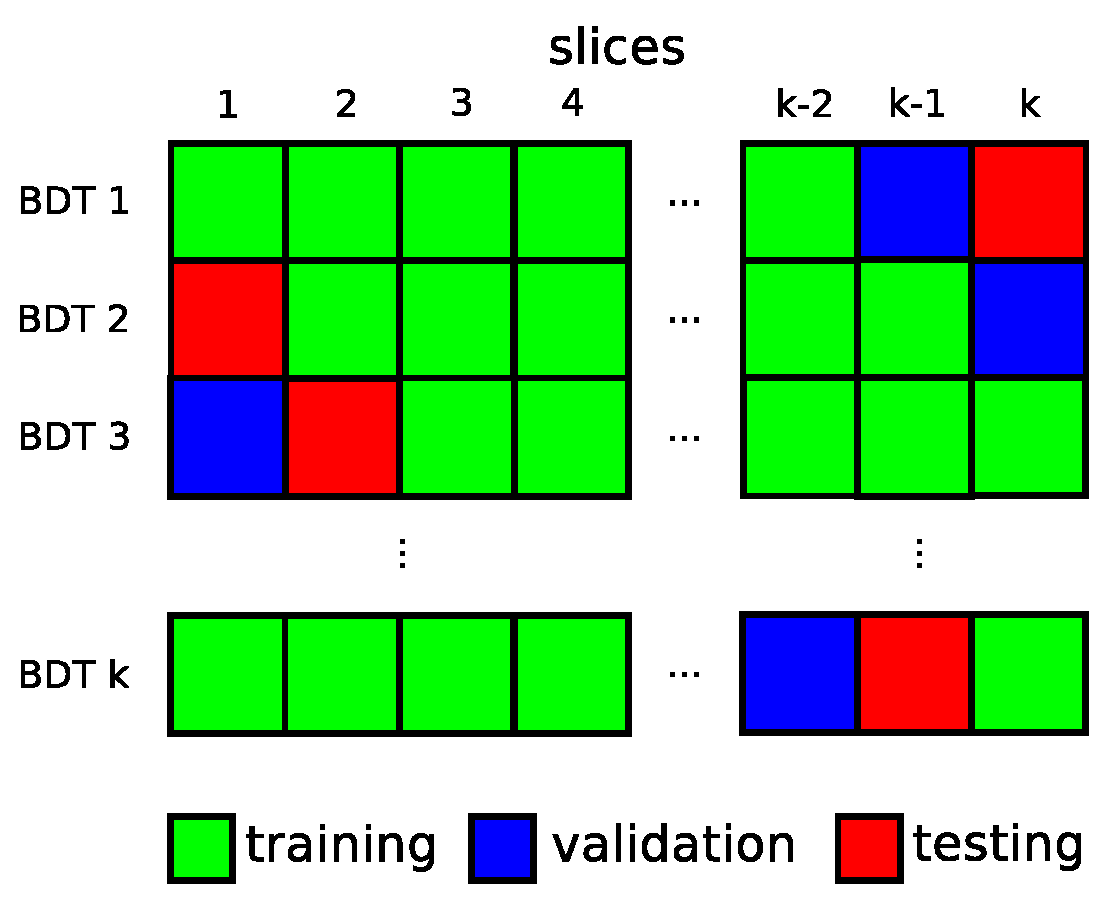
\includegraphics[width=0.6\textwidth]{./figures/mva/kfold-xval.eps}
    \caption{An illustration of the $k$-fold cross-validation scheme. The total set of simulated events is split into $k$ slices.
             All $k$ BDTs are trained, validated, and tested by using different combinations of the slices.}\label{fig:mva:kfold-xval}
\end{figure}

In the testing stage the $k$ BDTs need also be applied to data events.
The same approach as for simulated events could be used, where
a random number decides which BDT is used for which slices.
However, some scientists do not like the idea that data is treated randomly.
Also random numbers cannot be reproduced on all computer systems, even if they are seeded.
In this case for each data event the output of every BDT could be calculated
and an average over all BDT outputs could be built.
But this leads to another issues.
First, the simulated events and data events are treated in a different way.
Second, averaging over $k$ BDTs could lead to the effect, that events in border regions
are shifted towards the middle of the distribution, since the central limit theorem can be applied here.

In this thesis a third approach is used.
Every recorded data event in ATLAS is labeled with a unique number, the so-called event number.
This number is set once and not modified again.
The expression ``$\text{event number} \mod k$'' is used to split the data events into $k$ different slices.
This method was chosen because it treats data events similar to simulated events, but takes out the randomness of the splitting.
It needs to be checked that the data events are distributed equally in the different slices.
The distribution of of ``$\text{event number} \mod k$'' is shown in \cref{fig:mva:event_number_mod} for all
data events which pass the MVA selection.
Within two standard deviations the count in each slice agrees with the average.
Therefore this splitting procedure does not introduce slices of unequal size.

\begin{figure}[htb]
    \centering
    \includegraphics[width=0.7\textwidth]{./plots/mva/data_treatment/event_number_mod.pdf}
    \caption{Number of data events for each slice when splitting with ``$\text{event number} \mod k$'' is used.
             The plot shows data from the full 2015 and 2016 dataset which passed the MVA selection.}\label{fig:mva:event_number_mod}
\end{figure}

The three methods of data treatment are compared in \cref{fig:mva:data_treatment}.
Here the final BDTs which are selected in \cref{sec:mva:optimization} are used.
In the low-BDT-score regions in the boosted category the shift of events in the border region towards
the center when averaging over all BDTs can be seen.
Otherwise the methods agree within uncertainties.

\begin{figure}[htb]
    \centering
    \includegraphics[width=0.45\textwidth]{./plots/mva/data_treatment/VBF_SF_average_vs_split.pdf}
    \includegraphics[width=0.45\textwidth]{./plots/mva/data_treatment/VBF_DF_average_vs_split.pdf} \\
    \includegraphics[width=0.45\textwidth]{./plots/mva/data_treatment/BOOST_SF_average_vs_split.pdf}
    \includegraphics[width=0.45\textwidth]{./plots/mva/data_treatment/BOOST_DF_average_vs_split.pdf}
    \caption{Comparison of data treatment in $k$-fold cross-validation in the four MVA categories.
             The optimized BDTs from \cref{sec:mva:optimization} are used and are evaluated on the full
             2015 and 2016 dataset.}\label{fig:mva:data_treatment}
\end{figure}

\section{Optimization}\label{sec:mva:optimization}

For the optimization the VBF and boosted category are each split into
a \emph{same flavour} (SF, $ee$ and $\mu\mu$) and \emph{different flavour} (DF, $e\mu$ and $\mu e$) category,
based on the flavour of the final state leptons.
The optimization is done in each of those four categories individually, since the background composition for
different in each category.
In the VBF category only the VBF $\Htt$ sample is used for training and the boosted category uses only the ggF $\Htt$ sample as signal.
The other signal samples are discarded.
This decision was made even though the contributions of the VBF process in the boosted category and
the ggF process in the VBF category are not negligible.
Since the goal of this thesis is to measure the signal strength of $\Htt$ in the VBF- and ggF-production channel,
it makes sense to optimize the analysis for the production-channel-specific measurement.

The optimization is done in two steps.
First, the BDT hyperparameters are optimized. Here $58$ input variables are used, a full list can be found in \cref{cha:appendix_mva}.
However, such a high amount observables is not preferred, since the modelling of every observable needs to be tested.
Some observables are also highly correlated and provide only a tiny amount of new information.
Thus, the number of input variables for the BDTs is reduced in a second step, keeping only the variables which provide
the highest separation power.

\subsection{Figure of merit}\label{sub:figure_of_merit}

The separation power of a BDT can be assessed in different ways.
In this section several possible figures of merit are discussed,
which were considered for the estimation of the BDT performance.
These values are calculated on the validation set.

A common characteristic of a machine-learning model is the area under the receiver-operating characteristic (ROC) curve.
The ROC curve displays the rate of background rejection as a function of the rate of signal efficiency.
A larger area under the ROC curve indicates a better separation power.
The ROC curves are provided by TMVA\@.

Another figure of merit is the separation $\left<S^2\right>$, which is defined by~\cite{TMVA}
\begin{equation}
    \left<S^2\right> = \int_{-1}^1 \frac{{\left(\hat{y}_S(y) - \hat{y}_B(y)\right)}^2}{\hat{y}_S(y) + \hat{y}_B(y)} \dif y \,.
\end{equation}
The probability density functions of the output of the classifier are denoted as $\hat{y}_S$ and $\hat{y}_B$.
If the signal and background distribution have a complete overlap, the separation is zero.
Distributions with no overlap at all yield a separation of one.
The separation is also calculated by TMVA\@.

TMVA also provides a significance, which is calculated by
\begin{equation}
    Z_\text{TMVA} = \frac{\overline{y}_S - \overline{y}_B}{{\text{RMS}_S(y)}^2 + {\text{RMS}_B(y)}^2}
\end{equation}
Here $\overline{y}_{S}$ and $\overline{y}_{B}$ are the means of the classifier output for signal and background, respectively.
The root-mean-squares of the classifier output for signal and background are denoted as $\text{RMS}_S(y)$ and $\text{RMS}_B$.

Another way to calculate a significance is with \emph{binned significance}.
For this histograms with $10$ equidistant bins of the BDT distribution for signal and background is used.
If a bin contains less than $10$ background events, it is merged with its left neighbor (the most left bin is merged
with its right neighbor).
In each bin the significance is calculated with the asymptotic formula~\cite{CowanAsymSig}
\begin{equation}
    Z_\text{asym}(s, b) = \sqrt{2 \left( (s+b) \ln \left(1 + \frac{s}{b} \right) - s \right)} \,,
\end{equation}
where $s$ and $b$ are the expected signal and background yields.
The binned significance $Z_\text{binned}$ is the quadratic sum of the significances in the individual bins,
\begin{equation}
    Z_\text{binned} = \sqrt{\sum_i {Z_\text{asym}(s_i, b_i)}^2} \,.
\end{equation}
This significance is a simple approximation of the significance of the complete fit model, which is discussed in \cref{cha:fit}.

Of course the significance of the fit model can also be used to estimate the performance of a BDT\@.
This method is actually used for the optimization.
However, not the full fit model is applied.
Including all systematic variations (\cref{cha:systematics}) would need too much computing power to run the optimization in a reasonable timescale.
Therefore, the fit is done without the systematic variations, which is also denoted as \emph{stat.\ only fit} (``statistics only'').
The fit is performed with Asimov data (discussed in \cref{cha:fit}) to avoid biasing the optimization due to the observed data.

\subsection{Hyperparameters}\label{sub:mva:hyperparameters}

As mentioned before, in the first optimization different hyperparameters for the BDTs
are optimized.
The boosting algorithm, number of trees in the boosting, maximum depth of the tree, minimum number of events in the final nodes,
and the learning rate are varied in a grid scan.
The values which were for those parameters can be found in \cref{tab:mva:hpyerparameterscan}.
This leads to a total of 630 BDTs which need to be trained for each region.

\begin{table}[htpb]
    \centering
    \caption{Values of the BDT hyperparameters which are used in the first optimization step.
    The hyperparameters are explained in \cref{sec:bdt:hyperparameters}.}\label{tab:mva:hpyerparameterscan}
    \begin{tabular}{ll}
        \toprule
        Hyperparameter   & Values \\ \midrule
        BoostType   & AdaBoost, Grad (gradient boost) \\
        NTrees      & $50, 250, 500, 750, 1000$ \\
        MaxDepth    & $2, 3, 4, 5, 7, 10$ \\
        MinNodeSize & $\SI{1}{\percent}, \SI{5}{\percent}, \SI{10}{\percent}$ \\
        Shrinkage   & $0.05, 0.1, 0.2, 0.5$ \\
        AdaBoostBeta& $0.1, 0.5, 0.8$ \\
        \bottomrule
    \end{tabular}
\end{table}

\subsubsection{General observations}

Before the best BDT hyperparameters are chosen first a few general trends are discussed.
The significance depending on the boosting algorithm is shown in \cref{fig:mva:scan:boosttype}.
In all four regions the gradient-boosting algorithm yields on average a better significance than the AdaBoost algorithm.
For the VBF categories between 250 and 750 boosting iterations are preferred, in the boosted categories also BDTs with
1000 boosting iterations yield a comparable significance, as can be seen in \cref{fig:mva:scan:ntrees}.
%TODO finish

\begin{figure}[htb]
    \centering
    \begin{subfigure}[t]{0.45\textwidth}
        \includegraphics[width=\textwidth,page=1]{./plots/mva/scan/VBF_SF_setting_vs_binned_sig.pdf}
        \caption{VBF SF}
    \end{subfigure}
    \begin{subfigure}[t]{0.45\textwidth}
        \includegraphics[width=\textwidth,page=1]{./plots/mva/scan/VBF_DF_setting_vs_binned_sig.pdf}
        \caption{VBF DF}
    \end{subfigure}
    \begin{subfigure}[t]{0.45\textwidth}
        \includegraphics[width=\textwidth,page=1]{./plots/mva/scan/BOOST_SF_setting_vs_binned_sig.pdf}
        \caption{Boosted SF}
    \end{subfigure}
    \begin{subfigure}[t]{0.45\textwidth}
        \includegraphics[width=\textwidth,page=1]{./plots/mva/scan/BOOST_DF_setting_vs_binned_sig.pdf}
        \caption{Boosted DF}
    \end{subfigure}
    \caption{Significance of all trained BDTs depending on the boosting algorithm for each region.}~\label{fig:mva:scan:boosttype}
\end{figure}

\begin{figure}[htb]
    \centering
    \begin{subfigure}[t]{0.45\textwidth}
        \includegraphics[width=\textwidth,page=2]{./plots/mva/scan/VBF_SF_setting_vs_binned_sig.pdf}
        \caption{VBF SF}
    \end{subfigure}
    \begin{subfigure}[t]{0.45\textwidth}
        \includegraphics[width=\textwidth,page=2]{./plots/mva/scan/VBF_DF_setting_vs_binned_sig.pdf}
        \caption{VBF DF}
    \end{subfigure}
    \begin{subfigure}[t]{0.45\textwidth}
        \includegraphics[width=\textwidth,page=2]{./plots/mva/scan/BOOST_SF_setting_vs_binned_sig.pdf}
        \caption{Boosted SF}
    \end{subfigure}
    \begin{subfigure}[t]{0.45\textwidth}
        \includegraphics[width=\textwidth,page=2]{./plots/mva/scan/BOOST_DF_setting_vs_binned_sig.pdf}
        \caption{Boosted DF}
    \end{subfigure}
    \caption{Significance of all trained BDTs depending on the number of trees used in boosting for each region.}~\label{fig:mva:scan:ntrees}
\end{figure}

\begin{figure}[htb]
    \centering
    \begin{subfigure}[t]{0.45\textwidth}
        \includegraphics[width=\textwidth,page=3]{./plots/mva/scan/VBF_SF_setting_vs_binned_sig.pdf}
        \caption{VBF SF}
    \end{subfigure}
    \begin{subfigure}[t]{0.45\textwidth}
        \includegraphics[width=\textwidth,page=3]{./plots/mva/scan/VBF_DF_setting_vs_binned_sig.pdf}
        \caption{VBF DF}
    \end{subfigure}
    \begin{subfigure}[t]{0.45\textwidth}
        \includegraphics[width=\textwidth,page=3]{./plots/mva/scan/BOOST_SF_setting_vs_binned_sig.pdf}
        \caption{Boosted SF}
    \end{subfigure}
    \begin{subfigure}[t]{0.45\textwidth}
        \includegraphics[width=\textwidth,page=3]{./plots/mva/scan/BOOST_DF_setting_vs_binned_sig.pdf}
        \caption{Boosted DF}
    \end{subfigure}
    \caption{Significance of all trained BDTs depending on the maximum depth of the decision trees for each region.}~\label{fig:mva:scan:maxdepth}
\end{figure}

\begin{figure}[htb]
    \centering
    \begin{subfigure}[t]{0.45\textwidth}
        \includegraphics[width=\textwidth,page=4]{./plots/mva/scan/VBF_SF_setting_vs_binned_sig.pdf}
        \caption{VBF SF}
    \end{subfigure}
    \begin{subfigure}[t]{0.45\textwidth}
        \includegraphics[width=\textwidth,page=4]{./plots/mva/scan/VBF_DF_setting_vs_binned_sig.pdf}
        \caption{VBF DF}
    \end{subfigure}
    \begin{subfigure}[t]{0.45\textwidth}
        \includegraphics[width=\textwidth,page=4]{./plots/mva/scan/BOOST_SF_setting_vs_binned_sig.pdf}
        \caption{Boosted SF}
    \end{subfigure}
    \begin{subfigure}[t]{0.45\textwidth}
        \includegraphics[width=\textwidth,page=4]{./plots/mva/scan/BOOST_DF_setting_vs_binned_sig.pdf}
        \caption{Boosted DF}
    \end{subfigure}
    \caption{Significance of all trained BDTs depending on the minimum number events given as the fraction of all events for each region.}~\label{fig:mva:scan:minnodesize}
\end{figure}

\begin{figure}[htb]
    \centering
    \begin{subfigure}[t]{0.45\textwidth}
        \includegraphics[width=\textwidth,page=5]{./plots/mva/scan/VBF_SF_setting_vs_binned_sig.pdf}
        \caption{VBF SF}
    \end{subfigure}
    \begin{subfigure}[t]{0.45\textwidth}
        \includegraphics[width=\textwidth,page=5]{./plots/mva/scan/VBF_DF_setting_vs_binned_sig.pdf}
        \caption{VBF DF}
    \end{subfigure}
    \begin{subfigure}[t]{0.45\textwidth}
        \includegraphics[width=\textwidth,page=5]{./plots/mva/scan/BOOST_SF_setting_vs_binned_sig.pdf}
        \caption{Boosted SF}
    \end{subfigure}
    \begin{subfigure}[t]{0.45\textwidth}
        \includegraphics[width=\textwidth,page=5]{./plots/mva/scan/BOOST_DF_setting_vs_binned_sig.pdf}
        \caption{Boosted DF}
    \end{subfigure}
    \caption{Significance of all trained BDTs where the gradient boost algorithm was used depending on the learning rate for each region.}~\label{fig:mva:scan:shrinkage}
\end{figure}

\begin{figure}[htb]
    \centering
    \begin{subfigure}[t]{0.45\textwidth}
        \includegraphics[width=\textwidth,page=6]{./plots/mva/scan/VBF_SF_setting_vs_binned_sig.pdf}
        \caption{VBF SF}
    \end{subfigure}
    \begin{subfigure}[t]{0.45\textwidth}
        \includegraphics[width=\textwidth,page=6]{./plots/mva/scan/VBF_DF_setting_vs_binned_sig.pdf}
        \caption{VBF DF}
    \end{subfigure}
    \begin{subfigure}[t]{0.45\textwidth}
        \includegraphics[width=\textwidth,page=6]{./plots/mva/scan/BOOST_SF_setting_vs_binned_sig.pdf}
        \caption{Boosted SF}
    \end{subfigure}
    \begin{subfigure}[t]{0.45\textwidth}
        \includegraphics[width=\textwidth,page=6]{./plots/mva/scan/BOOST_DF_setting_vs_binned_sig.pdf}
        \caption{Boosted DF}
    \end{subfigure}
    \caption{Significance of all trained BDTs where the AdaBoost algorithm was used depending on the learning rate for each region.}~\label{fig:mva:scan:adaboostbeta}
\end{figure}

\FloatBarrier{}

\subsubsection{Result of optimization}

The overtraining of a BDT can be estimated by using the \emph{Kolmogorov--Smirnov test}~\cite{KSk, KSs} (KS-test).
Here the BDT output of training and validation set is compared for both the signal and background distribution.
The KS-test yields a probability between zero and one, where one indicates perfect agreement and zero no agreement at all.
Only BDTs which yield a KS-test probability for both signal and background distribution above $0.4$ are considered. %TODO motivate with ks sig vs bkg, plots in backup
The BDT with the best significance is selected for each region, the hyperparameters of the best performing BDTs are
listed in \cref{tab:mva:bestparams}.
The distributions of the BDTs are shown in \cref{fig:mva:scan:bdts}.
%TODO discuss distributions

\begin{table}[htpb]
    \centering
    \caption{Hyperparameters of the best performing BDTs in each region.}\label{tab:mva:bestparams}
    \begin{tabular}{@{}lccccc@{}}
        \toprule
        Region     & Type & NTrees & MaxDepth & MinNodeSize & LearnRate \\ \midrule
        VBF SF     & Grad & 250    & 2        & 1\,\%       & 0.1          \\
        VBF DF     & Grad & 250    & 5        & 10\,\%      & 0.05         \\
        Boosted SF & Grad & 500    & 4        & 5\,\%       & 0.05         \\
        Boosted DF & Grad & 250    & 5        & 5\,\%       & 0.1          \\
        \bottomrule
    \end{tabular}
\end{table}

\begin{figure}[htb]
    \centering
    \begin{subfigure}[t]{0.49\textwidth}
        \includegraphics[width=\textwidth]{./plots/mva/scan/VBF_SF_bdt_output.pdf}
        \caption{VBF SF}
    \end{subfigure}
    \begin{subfigure}[t]{0.49\textwidth}
        \includegraphics[width=\textwidth]{./plots/mva/scan/VBF_DF_bdt_output.pdf}
        \caption{VBF DF}
    \end{subfigure}
    \begin{subfigure}[t]{0.49\textwidth}
        \includegraphics[width=\textwidth]{./plots/mva/scan/BOOST_SF_bdt_output.pdf}
        \caption{Boosted SF}
    \end{subfigure}
    \begin{subfigure}[t]{0.49\textwidth}
        \includegraphics[width=\textwidth]{./plots/mva/scan/BOOST_DF_bdt_output.pdf}
        \caption{Boosted DF}
    \end{subfigure}
    \caption{Distributions of the best performing BDTs in the hyperparameter optimization for signal and background and the training and validation set.}~\label{fig:mva:scan:bdts}
\end{figure}

\subsection{Input variables}\label{sub:mva:input_variables}

\begin{table}[htpb]
	\centering
	\caption{List of observables which are used as input variables for the BDTs in the VBF category.}\label{tab:mva:variables:vbf}
	\begin{tabular}{lcc}
		\toprule
		Observable                                  & SF        & DF        \\ \midrule
		$m_\text{MMC}$                              & $\bullet$ & $\bullet$ \\
		$\min \Delta \eta (\ell\ell, \text{jets})$  & $\bullet$ & $\bullet$ \\
		$m_\text{jj}$                               & $\bullet$ & $\bullet$ \\
		$\Delta R(\ell,\ell)$                       & $\bullet$ & $\bullet$ \\
		$n_\text{jets}$                             & $\bullet$ & $\bullet$ \\
		$\etmiss$ $\Phi$ centrality                 & $\bullet$ & $\bullet$ \\
		$\pt^\text{total}$                          & $\bullet$ & $\bullet$ \\
		$\etmiss$                                   & $\bullet$ &           \\
		$\min \Delta R (\ell_1, \text{jets})$       & $\bullet$ &           \\
		$\min \Delta R (\ell_0, \text{jets})$       &           &           \\
		\bottomrule
	\end{tabular}
\end{table}

\begin{table}[htpb]
    \centering
	\caption{List of observables which are used as input variables for the BDTs in the boosted category.}\label{tab:mva:variables:boost}
    \begin{tabular}{lcc}
        \toprule
        Observable                                  & SF        & DF        \\ \midrule
        $m_\text{MMC}$                              & $\bullet$ & $\bullet$ \\
        $m_{\ell\ell}$                              & $\bullet$ & $\bullet$ \\
        $\etmiss$                                   & $\bullet$ &           \\
        $\Delta R (\ell, \ell)$                     & $\bullet$ & $\bullet$ \\
        $m_{\tau\tau,\text{j}_0} $                  &           & $\bullet$ \\
        $\etmiss / \pt^{\ell_1}$                    &           & $\bullet$ \\
        Sphericity                                  &           & $\bullet$ \\
        $m_\text{T}^{\ell_0}$                       &           & $\bullet$ \\
        $\eta_{\ell_0}$                             &           & $\bullet$ \\
        $\min \Delta \eta (\ell\ell, \text{jets})$  &           & $\bullet$ \\
        \bottomrule
    \end{tabular}
\end{table}


\section{Modeling checks}\label{sec:mva:}

\section{Optimal Binning}\label{sec:mva:binning}
%TODO move to statistical analysis
